\documentclass{beamer}
\usepackage{wrapfig}
\usepackage{commath}
\usepackage{braket}
%\usepackage{physics}
\usepackage{amsmath,amssymb,amsfonts,scalerel,stackengine}
\usepackage{mathpazo}
\usepackage{subcaption}
\usepackage{multicol}
\usepackage{mathtools}
\usepackage[makeroom]{cancel}
\usepackage{lipsum}
\usepackage{tikz}
\usetikzlibrary{quantikz}
\usepackage{bm}


%\usepackage{sectsty}
\usepackage[export]{adjustbox}
\usetheme{Boadilla}
\usefonttheme[onlymath]{serif} 
\setbeamertemplate{navigation symbols}{}
\usepackage{graphicx}
% NOTE: use biber and cite with \footfullcite{key}
\usepackage[style=numeric-comp, sorting=none]{biblatex}
\usepackage{amsmath}
\usepackage{ulem}
\addbibresource{references_presentation.bib}
\setbeamertemplate{footline}
{
  \leavevmode%
  \hbox{%
  \begin{beamercolorbox}[wd=.2\paperwidth,ht=2.25ex,dp=1ex,center]{author in head/foot}%
    \usebeamerfont{author in head/foot} \insertshortdate{}%
  \end{beamercolorbox}%
  \begin{beamercolorbox}[wd=.6\paperwidth,ht=2.25ex,dp=1ex,center]{title in head/foot}%
    \usebeamerfont{title in head/foot}\insertshorttitle
  \end{beamercolorbox}%
  \begin{beamercolorbox}[wd=.2\paperwidth,ht=2.25ex,dp=1ex,center]{date in head/foot}%
 
    \insertframenumber{} / \inserttotalframenumber\hspace*{1ex}
  \end{beamercolorbox}}%
  \vskip0pt%
}
\DeclareMathOperator*{\argmin}{argmin}
\renewcommand*{\bibfont}{\normalfont\tiny}
\renewcommand{\footnotesize}{\tiny}
\title{Variational Monte-Carlo for strongly correlated bosons in continuous space}
\author{Giorgio Facelli}
\date{28/06/2023}

\setbeamercolor{normal text}{fg=black}
\begin{document}

\begin{frame}[plain]
    \titlepage
    \begin{center}
      Hosting group: CQSL lead by Prof.\ Giuseppe Carleo \\
      Supervision: Gabriel Pescia
      \end{center}
\end{frame}

\begin{frame}{Contents}
  \begin{enumerate}
    \item \large Introduction
    \item \large Methods
    \begin{enumerate}[I]
      \item VMC approach
      \item How to implement periodic boundary conditions
      \item Gaussian cores
      \item NQS architecture: MPNN
      \item Relevant physical quantities
    \end{enumerate} 
    \item \large Results
    \begin{enumerate}[I]
      \item MPNN performance
      \item Ground-state properties: phases of matter, 2D geometry
    \end{enumerate}
    \item \large Conclusions
  \end{enumerate}
    %\begin{block}
    %    {Dummy Block}
    %    \lipsum[1]
    %\end{block}
\end{frame}

%%%%%%%%%%%%%%%%%%%%%%%%%%%%%%%%%%

\begin{frame}{Introduction}
\begin{itemize}
\item[-]Many-body quantum systems very difficult to study - \textit{ab initio} simulations often 
unfeasible (e.g. $N$ constituents with $d$ d.o.f $\implies \text{dim}(\mathcal{H}) = d^N$). \\
\vspace{0.5cm}
\item[-]\textbf{Possible solution:} \\
Machine Learning (ML) techniques + MC statistical methods. \\
\textbf{ANNs} = Universal function approximators. Can also encode relevant physical symmetries in the architectures. \\
\vspace{0.5cm}
\item[-]Recent \textbf{state-of-the-art} has allowed to study systems with both discrete and continuous degrees of freedom \cite{carleo_2017, hibat-allah_2020, choo_2018,pescia_2022, pescia_2023, pfau_2020}. \\
\end{itemize}
\vspace{0.5cm}
In this study: 2D boson particles interacting through a gaussian core potential.
\end{frame}

%%%%%%%%%%%%%%%%%%%%%%%%%%%%%%%%%%

\begin{frame}{Variational Monte-Carlo (VMC)}
Exploits the \textit{variational principle}, which states that the ground-state $\ket{\Psi_0}$ minimizes 
the energy:
\begin{equation*}
  \ket{\Psi_0} = \argmin_{\ket{\Psi}}\biggr[\dfrac{\braket{\Psi|\hat{H}|
  \Psi}}{\braket{\Psi|\Psi}}\biggr]
\end{equation*}
Given an ansatz $\ket{\Psi(\bm{\theta})}$, the parameters are optimized so as to reach the minimum in 
energy.\\
\textbf{Observables:} Almost every observable can be estimated as a stochastic expectation value over its 
\textit{local} counterpart:
\begin{equation*}
\braket{\hat{O}} = E_{\Pi(\bm{x})}\big[O_{\text{loc}}(\bm{x})\big]\text{   where   }
O_\text{loc}(\bm{x}) = \int \,d\bm{x}' O_{\bm{xx}'} \dfrac{\Psi(\bm{x}')}{\Psi(\bm{x})}
\end{equation*}
over the distribution $\Pi(\bm{x}) = \frac{|\Psi_{\bm{\theta}}(\bm{x})|^2}{\int \,d\bm{y} |\Psi_{\bm{\theta}}(\bm{y})|^2}$.
\end{frame}
  
%%%%%%%%%%%%%%%%%%%%%%%%%%%%%%%%%%

\begin{frame}{Periodic Boundary Conditions (PBCs)}
PBCs allow to access the bulk properties of a system. For a simulation box of size 
$\bm{L} = (L_1,...,L_d)$ we map each vector $\bm{x}_i$ describing said system into a periodic representation:
\begin{equation*}
  \bm{x}_i \longmapsto \bm{r}_i=\Biggr(\sin\biggr(\dfrac{2\pi}{\bm{L}}\bm{x}_i\biggr), \cos\biggr(\dfrac{2\pi}{\bm{L}}\bm{x}_i\biggr)\Biggr)
\end{equation*}
To compute the euclidean distance between two particles, we adopt the \textit{minimum image} convention:
\begin{equation*}
  d(i,j) = \biggr\lVert \bm{x}_i -\bm{x}_j - \bm{L}\left\lfloor \dfrac{\bm{x}_i -\bm{x}_j}{\bm{L}}\right\rceil \biggr\rVert
\end{equation*}
In the NQS architecture we will instead use the differentiable variant:
\begin{equation*}
  d_{\sin}(i,j) = \biggr\lVert \sin\biggr(\dfrac{\pi(\bm{x}_i-\bm{x}_j)}{\bm{L}}\biggr)\biggr\rVert
\end{equation*}

\end{frame}

%%%%%%%%%%%%%%%%%%%%%%%%%%%%%%%%%%

\begin{frame}{Gaussian cores}
In this study, we investigate the physical properties of bosons with spin zero in PBCs interacting through a 
repulsive \textbf{gaussian core} potential in 2D. The entire Hamiltonian reads:
\begin{equation*}
  \begin{split}
  \hat{H} &= \hat{T}+\hat{V}=-\dfrac{\hbar^2}{2m}\sum_{i=1}^N\vec{\nabla}^2_i+\varepsilon\sum_{i<j}^N\exp\biggr(-\dfrac{d(i,j)}{2\sigma^2}\biggr) = \\ 
      &= -\dfrac{\Lambda}{2}\sum_{i=1}^N\vec{\nabla}^2_i+\sum_{i<j}^N\exp\biggr(-\dfrac{d(i,j)}{2}\biggr)
\end{split}
\end{equation*} 
where in the last equality we simplified the expression by renormalizing the coordinates by $\sigma^2$ and defining $\Lambda=\hbar^2/m\varepsilon\sigma^2$.

\end{frame}

%%%%%%%%%%%%%%%%%%%%%%%%%%%%%%%%%%

\begin{frame}{NQS architecture (1)}
Message-passing neural networks (MPNNs) to represent data as graphs (nodes+edges). Able to encode 
symmetries \cite{gilmer2017neural}. 
\begin{columns}
\begin{column}{0.46\textwidth}
We transform the data by feeding it into a composition of $\mathcal{N}$ graphs. 
We are interested in spatial structure of system $\implies$ nodes: 1-body coord's / edges: 2-body coord's.
For the $\mu$-th graph:
{\small
\begin{equation*}
  \begin{split}
  \bm{n}_i^{(\mu)} &= \biggr(\bm{r}_i, \bm{h}_i^{(\mu)}\biggr) \\
  \bm{e}_{ij}^{(\mu)} &= \biggr(\bm{r}_{ij},d_{\sin}(i,j), \bm{h}_{ij}^{(\mu)}\biggr)
  \end{split}
\end{equation*}
}
\end{column}

\begin{column}{0.5\textwidth}
\begin{figure}
  \centering
  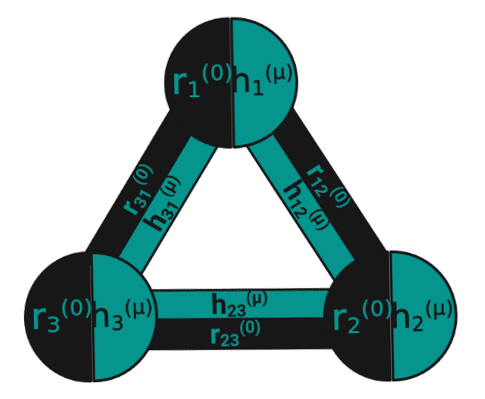
\includegraphics[scale=0.3]{figures/GNN_diagram.png}
  \caption{Schematic of three-particle MPNN, with nodes (circles) and edges (connections).}
  \label{fig:gnn_diagram}
\end{figure}
\end{column}

\end{columns}
\end{frame}

\begin{frame}{NQS architecture (2)}
\textit{Hidden} nodes and edges:
\begin{equation*}
  \bm{h}_{i}^{(\mu)} = \bm{f}\biggr(\bm{n}_i^{(\mu-1)}, \sum_{i\neq j} \bm{m}_{ij}^{(\mu)}\biggr), \hspace{0.5cm} \bm{h}_{ij}^{(\mu)} = \bm{g} \biggr(\bm{e}_{ij}^{(\mu-1)}, \bm{m}_{ij}^{(\mu)}\biggr)
\end{equation*}
where $\bm{m}_{ij}^{(\mu)} = \bm{\phi}\big(\bm{e}_{ij}^{(\mu-1)}\big)$. The functions $\bm{f},\bm{g},\bm{\phi}$ are simple feed-forward artificial 
neural networks. \\
\textbf{Permutation equivariance:} ensured by taking same initial hidden variables for all $(i,j)$. In summary, we construct the ansatz by transforming the particle positions into backflow coordinates 
$\bm{\tilde{x}}_i = \text{MPNN}(\bm{x})_i$ and feed them into a final MLP:
\begin{equation*}
  \log[\Psi_{\bm{\theta}}(\bm{x})] = \sum_i \bm{\rho}(\bm{\tilde{x}}_i) = \sum_i \bm{\rho}(\text{MPNN}(\bm{x})_i)
\end{equation*}
\end{frame}

\begin{frame}{Investigating the physical structure}
\begin{columns}

\begin{column}{0.5\textwidth}
Radial correlation function:
\begin{equation*}\label{eq:rad_corr}
  g_2(\bm{r}) = \dfrac{1}{N\rho}\braket{\sum_{i\neq j}^N\delta(\bm{r}-\bm{r}_{ij})}
\end{equation*}
\end{column}

\begin{column}{0.5\textwidth}
Pair correlation function:
\begin{equation*}\label{eq:pair_corr}
  g_2(r) = \dfrac{1}{N\rho}\dfrac{1}{4\pi r^2}\braket{\sum_{i\neq j}^N\delta(r-r_{ij})}
\end{equation*} 
\end{column}

\end{columns}
\vspace{0.5cm}
Both give us insight on the probability to find a particle in position $\bm{r}\text{ (or } r$) given a particle at the origin. \\
\vspace{0.5cm}
The structure factor, useful in determining scattering properties, can be used to infer the structural arrangement. It is given by:
\begin{equation*}
S(\bm{q}) = \dfrac{1}{N}\biggr|\braket{\sum_{i=1}^N e^{-i\bm{q}\cdot\bm{r}_i}}\biggr|^2
\end{equation*}
\end{frame}

\begin{frame}{Results - MPNN performances}
$N=16;\hspace{4pt}\Lambda=1/30;\hspace{4pt}\text{SGD}+\text{SR};\hspace{4pt}\text{samples}=5\cdot10^3$.
Firstly, we study the impact of number of graphs and number of hidden layers in the architecture.
\begin{columns}

  \begin{column}{0.55\textwidth}
  \begin{figure}
    \centering
    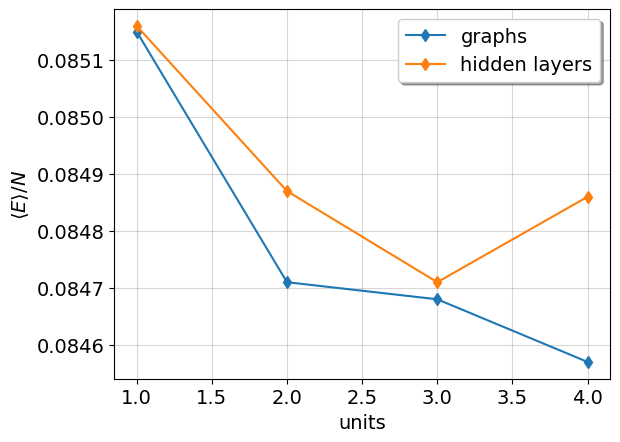
\includegraphics[scale=0.4]{figures/gs_energy_diff_graphs_and_lyrs.png}
    \caption{Ground-state energy at $\rho=1/9$, for different number of graphs, hidden layers.}
  \end{figure}
  \end{column}

  \begin{column}{0.45\textwidth}
    \begin{table}[H]
      \centering
      \caption{Energy per particle for $\rho = 4/9, 1/9$ with and without applying LN after each activation 
      layer in the MPNN architecture.}
      \begin{tabular}{|c|c|c|}
          \hline
          & No \textbf{LN} & \textbf{LN} \\
          \hline
          \hline
          $\rho = 4/9$ & $1.00498$ & $1.00403$ \\
          \hline
          $\rho = 1/9$ &  $0.08534$ & $0.08515$ \\
          \hline
      \end{tabular}
  
  \end{table}
  \end{column}

\end{columns}
\end{frame}

\begin{frame}{Results - phases of matter}
Investigation of the average particle density's impact on the \textbf{phases of matter}
\begin{figure}
\centering
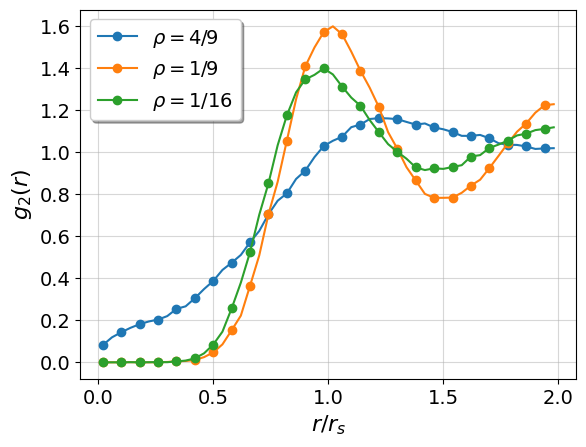
\includegraphics[scale=0.5]{figures/corr_func_diff_densities.png}
\caption{Pair correlation function at three different densities.}
\end{figure}
\end{frame}

\begin{frame}{Results - geometry of the simulation box (1)}
  $\Lambda = 1/100$. Change of the aspect ratio of the simulation box \\
  $\implies$ \textbf{relaxation} in energy up to $a=2/\sqrt{3}$.
  \begin{columns}
    \begin{column}{0.5\textwidth}
      \begin{figure}[H]
          \centering
          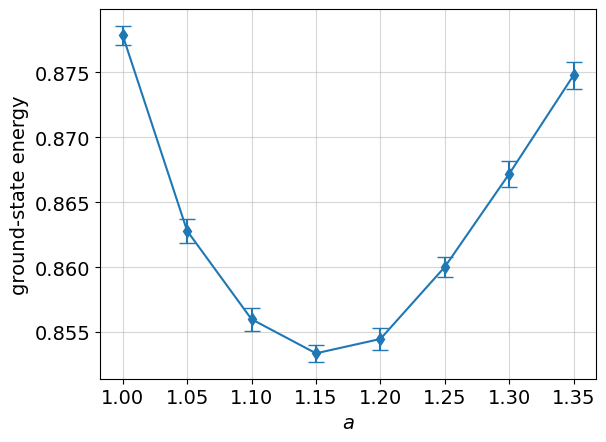
\includegraphics[width=1.0\textwidth]{figures/gs_energy_against_a_iters=2000.png}
          \caption{Ground-state energy against aspect ratio. Minimum in $a=2/\sqrt{3}$.}
      \end{figure}
    \end{column}

    \begin{column}{0.5\textwidth}
    \begin{figure}[H]
          \centering
          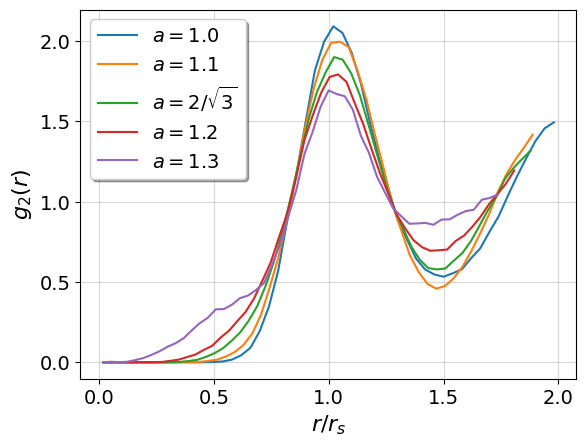
\includegraphics[width=1.0\textwidth]{figures/corr_func_diff_a_2.png}
          \caption{Pair correlation function at different values of the aspect ratio.}
    \end{figure}
    \end{column}
  \end{columns}
\end{frame}

\begin{frame}{Results - geometry of the simulation box (2)}
  Radial correlation function localizes in well-defined \textbf{clusters} for higher $a$ (two-particle unit 
  cell becomes clearly visible). Structure factor also indicates a more rigid structure.
  \begin{columns}
    \begin{column}{0.5\textwidth}
      \begin{figure}
        \centering
        \vspace{-0.75cm}
        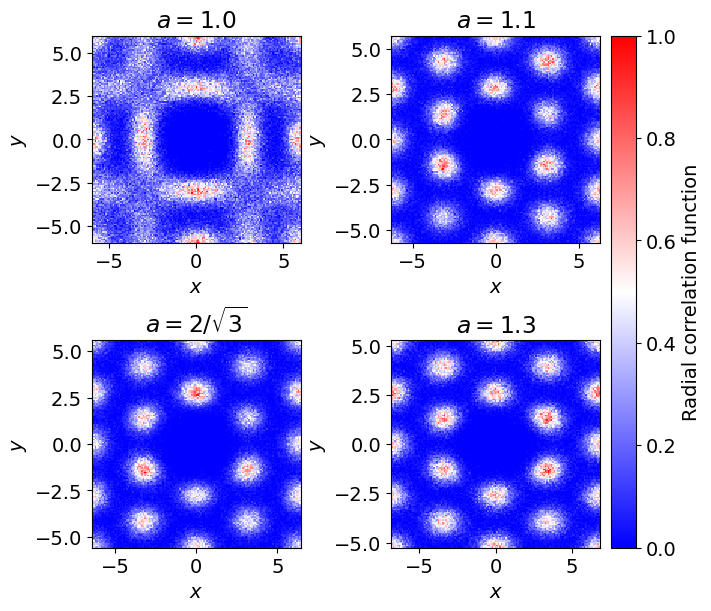
\includegraphics[scale=0.35]{figures/pair_corr_func_xy_diff_a_2.png}
        \caption{Radial correlation function for different aspect ratios.}
      \end{figure}
    \end{column}

    \begin{column}{0.5\textwidth}
      \begin{figure}
        \centering
        \vspace{-0.75cm}
        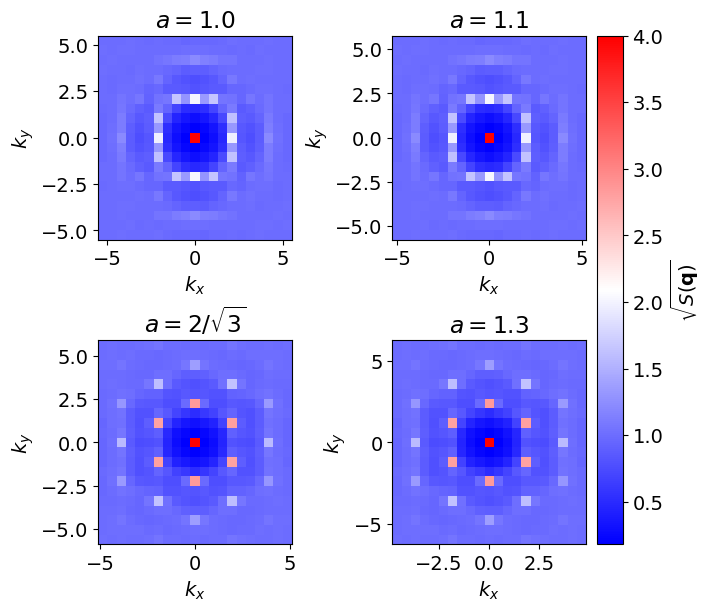
\includegraphics[scale=0.35]{figures/structure_factor_diff_a.png}
        \caption{Square root of the structure factor for different aspect ratios.}
      \end{figure}
    \end{column}
  \end{columns}
\end{frame}

\begin{frame}{Conclusions}
\begin{itemize}
  \item[-]\textbf{MPNN} Neural Quantum States can \textbf{accurately} describe a continuous-variable system. 
  Also largely \textbf{flexible}, no matter the physical parameters or the emergent structure of the system.\\
  \vspace{0.3cm}
  \item[-]Gaussian cores in \textbf{superfluid} phase at high and low densities. They instead 
  self-assemble into a \textbf{crystalline} structure at intermediate densities ($\rho=1/9$).\\
  \vspace{0.3cm}
  \item[-]Crystal is even more \textbf{rigid} when the environment conforms to the aspect ratio of the unit cell.  
\end{itemize}
\vspace{2cm}
\begin{center}
{\huge  Thank you!}
\end{center}
\end{frame}
\begin{frame}{References}
  \printbibliography
\end{frame}
\end{document}

